 \documentclass[12pt]{MUNThesis}
%set MUN Thesis Guidelines margins
\usepackage[left=3.8cm, right=2.5cm, top=3cm, bottom=3cm]{geometry}

%lists package and bullet formats
\usepackage{paralist,hyperref}
\usepackage{bbding}
%enhanced graphics support
\usepackage{graphicx}
%formatting for websites and e-mail addresses
\usepackage{url}
%pageheaders and footers in LaTeX2e
\usepackage{fancyhdr}
%footnote options
\usepackage{footmisc}
%algorithms
\usepackage{algorithmic}
%source code printer
\usepackage{listings}
%read/write verbatim TeX code
\usepackage{fancyvrb}
\usepackage{cite}
\usepackage[acronym, toc]{glossaries}
\makeglossaries
	
%might be superfluous; better math support
\usepackage{amsmath}
%rotating figures, tables
\usepackage{rotating}
%fancier tables!
\usepackage{booktabs}
%sci notation support
\usepackage[separate-uncertainty = true,multi-part-units=single]{siunitx}
%\usepackage{chapterbib}

\usepackage[version=3]{mhchem}

%You can add in your own shortcuts here.  I've put in some common ones I use.
\newcommand{\eg}{\emph{e.g.}}
\newcommand{\cm}{cm$^{-1}$}

%Uncomment one or more of the following to use different scripts
%CJK commands
%Simplified Chinese
%\newcommand{\zhs}[1]{\begin{CJK}{UTF8}{gbsn}#1\end{CJK}}
%Traditional Chinese
%\newcommand{\zht}[1]{\begin{CJK}{UTF8}{bsmi}#1\end{CJK}}
%Japanese Kanji, Hiragana and Katakana
%\newcommand{\nippon}[1]{\begin{CJK}{UTF8}{ipam}#1\end{CJK}}
%Korean Hangul
%\newfontfamily\hangul{Batang}
%Korean Hanja
%\newcommand{\hanja}[1]{\begin{CJK}{UTF8}{bsmi}#1\end{CJK}}
 
%package conflicts - only one may be activated
%\usepackage{arabtex}
%\usepackage{devanagari}


%enable endnotes - if you wish to enable endnotes, remove the % sign at the start of the following line
%\usepackage{endnotes}
%\let\footnote=\endnote



%THIS IS WHERE YOU ENTER THE TITLE OF YOUR THESIS
\title{Continuous Degeneracy and Magnetization Process
in the 3D FCC Kagome Lattice with the
Dipole-Dipole Interaction}

%THIS IS WHERE YOU ENTER YOUR NAME
\author{Andrew Way}

%THIS IS WHERE YOU ENTER THE NAME OF YOUR DEGREE
\deg{Bachelor of Science}

%THIS IS WHERE YOU ENTER THE NAME OF YOUR DEPARTMENT, SCHOOL, or FACULTY
\fac{Department of Physics}

%THIS IS WHERE YOU ENTER THE DATE YOU SUBMITTED YOUR THESIS OR DISSERTATION
\date{May 2017}

%THIS IS WHERE YOU ENTER THE YEAR OF GRADUATION 
\copyrightyear{2017}


%no paragraph indentation
%\setlength\parindent{0pt}
\newtheorem{theorem}{Theorem}[section]
\newtheorem{definition}{Definition}[section]
\newtheorem{lemma}{Lemma}[section]
\newtheorem{notation}{Notation}[section]
\begin{document}
\muntitlepage

%set the hierarchical drilldown to 3
\setcounter{secnumdepth}{3} \setcounter{tocdepth}{3}

%set pagination to Roman numerals and begin at page i
\pagenumbering{roman} \setcounter{page}{1}

%include the abstract.tex file
%%-------------Abstract-----------------
\doublespacing
\setlength{\topmargin}{-.5in}
\chapter*{Abstract}


\addcontentsline{toc}{chapter}{Abstract}


%enter text for the abstract below

Results are presented on analytic and computational analyses of the spin states associated with ABC stacked
kagome planes of magnetic ions with only long-range dipole-dipole interactions. Extending previous work on
the 2D kagome system, where six-fold discrete degeneracy of the ground state was revealed [1], we show that
the 3D FCC kagome lattice exhibits a continuous degeneracy characterized by just six sub-lattice spin vectors
and two spherical angles. Thermal fluctuations are shown to lift this degeneracy in an order-by-disorder
process. Degaussing the lattice with a magnetic field applied along directions of high symmetry also results
in lifting the continuous degeneracy to a subset of states from the original set of ground states, characterized by a single parameter. This lattice type is a model for the magnetic Mn ions in IrMn3, the most popular compound used as the antiferromagnetic pinning layer in hard-drive spin valve structures [2]. Analysis of these spin states is relevant for a deeper understanding of magnetic and thermal stability at surfaces and in thin films of IrMn3.




%include the acknowledgments.tex file
%%-----------Acknowledgements---------------
\chapter*{Acknowledgements}
\addcontentsline{toc}{chapter}{Acknowledgments} 


%enter text for the acknowledgements below

At a minimum you must acknowledge the funding sources for your work.

%%-----------Table of Contents------------------
\renewcommand{\contentsname}{Table of Contents}
\tableofcontents{}
\addcontentsline{toc}{chapter}{Table of Contents}
%%------------List of Tables----------------------
\listoftables{}
\addcontentsline{toc}{chapter}{List of Tables}
%%------------List of Figures----------------------
\listoffigures{}
\addcontentsline{toc}{chapter}{List of Figures}
%%------------List of Abbreviations----------------------
%\printglossaries
\addcontentsline{toc}{chapter}{List of Abbreviations and Symbols}
\chapter*{List of Abbreviations and Symbols}
If you don't have a list of abbreviations, then you don't need to include this file and you can comment out the corresponding lines in your main .tex file.  For example, if this file just defined a couple of terms such as AFM, then you wouldn't necessarily need this.

If you do have abbreviations to define, then you will probably set them up in a table like this:

\begin{tabular}{ll}
  $E$ & energy\\
  $\vec{E}$ & electric field\\
  EFMS & Erika\\
\end{tabular}




%change single space to double space
\doublespacing
%maintain Roman numerals on the previous page
\clearpage
%set pagination to Arabic
\pagenumbering{arabic} 

%include the other .tex files 
\chapter{Introduction (can be a more descriptive title)}\label{ch:intro}
\setcounter{secnumdepth}{3} \pagenumbering{arabic}
\setcounter{page}{1} \pagestyle{myheadings}
\markboth{}{}\markright{} \rhead{\thepage} \setcounter{page}{1}
\pagestyle{myheadings} \pagenumbering{arabic} \rhead{\thepage}
\setcounter{page}{1}

\section{A section}

Your first step in using this template should be to rename the folder and main .tex file to something involving your name.  That will help me to keep track of the various theses I'm reading!


\subsection{A subsection about getting organized}\label{sect:org}

Then start creating an outline for your thesis.  If you already have chapters written as papers, perhaps you should be using the ``MUN\_Thesis\_multiple\_bibliographies'' template.

To create the outline, create the chapters and write in all of the sections, subsections, etc. Then send that file to me so that I can look it over.  This is particularly important for the introduction or background chapter.  If we agree on the scope of your thesis up front, you will save yourself time later.

\subsection{Scope}

The main purpose of the first section is to provide the context for your work.  What have other people done in this area, with these techniques?  What background information does a somewhat general reader (\eg\ chemist just starting a graduate program) need to know in order to appreciate and understand your work?

\section{Another section}

As you write your thesis, be sure to use labels and references for your tables, figures, equations, chapters, etc.  This is another important aspect of getting organized, a topic which was discussed in Section \ref{sect:org}.  Be sure to pick unique labels.  For example, ``raman'' or "afm" are probably not good labels, since you will probably have multiple figures, tables, equations, and sections which could carry those labels. Your whole thesis, including material in, for example, Appendix \ref{app:spect}, will have one common list of labels.

Note the pretty quotes around raman and the not-so-pretty quotes around afm.  See the .tex file to know how to do this.

\subsection{Some technical details}

Pretty much all equations should be set off and numbered rather than included inline.  The Tabor coefficient, $\mu$, can be used to determine whether material deformation should be taken into account.\cite{tabor}
%
\begin{equation}
\label{eqn:tabor}
\mu = \left[ \frac{R(\Delta\gamma)^2}{E^{*2} \sigma^3} \right]^{1/3}
\end{equation}
%
where $R$ is the indenter tip radius, $\Delta\gamma$ is the work of adhesion, $\sigma$ is the separation, and $E^*$ is defined as
%
\begin{equation}
\label{eqn:Estar}
\frac{1}{E^*} = \frac{1-\nu_\text{tip}^2}{E_\text{tip}} + \frac{1-\nu_\text{sample}^2}{E_\text{sample}}
\end{equation}
%
$\nu_\text{tip}$ is....

Note that the equations are part of a paragraph.  Check how this is done in the .tex file, by not leaving blank lines before or after the equation.  Also, note that the font used in the text for the symbols is the same as that used in the equation, and that text in the equation doesn't need to be in math mode.
\chapter{Methods}\label{ch:expt}


\section{Substrate preparation}

This is a good chapter to write continuously throughout your degree program.  It will be easier to write up a procedure while it's fresh in your mind, and that way you won't be hunting down an instrument model or consumables supplier later.

If you are varying several parameters in your procedure, you may want to tabulate your different combinations.  Table \ref{icecream} summarizes ice cream texture characteristics used by McGhee et al\cite{McGhee}.

\begin{table}[!htbp]
\caption[Note how this caption is at the top of the table.  Also, note that the caption in the List of Tables doesn't include the reference number.]{Note how this caption is at the top of the table.  Also, note that the caption in the List of Tables doesn't include the reference number.\cite{McGhee}. \label{icecream}}

\centering
\begin{tabular}{lc}
 Characteristic& Mean value\\\hline
Icy	 &4.63\\
Crumbly	 &4.75\\
Fluffy	 &4.58\\
Gummy	 &4.71\\
Sandy	 &4.58\\
Soggy	 &4.29\\
Weak body&3.92\\
\end{tabular}
\end{table}

\subsection{Lots of chemicals}

I used \ce{K2HPO4}, \ce{KH2PO4.2H2O}, and other salts containing \ce{PO4^{3-}} ions.  Best of all, I didn't write out those chemical formula by hand using subscripts and superscripts.  See the .tex file to find out how!

\section{Atomic Force Microscopy}

A picture is worth a thousand words!  If you are creating your own schematics, consider using a program which will saves images in a precise and generally readable format such as SVG.  Inkscape will do that for you and is open source.

There are many public domain and other freely reproducible images available on the Wikimedia Commons.  You can also easily get permission to reuse a figure from most journals through RightsLink.

\begin{figure}[!hbtp]
\centering
    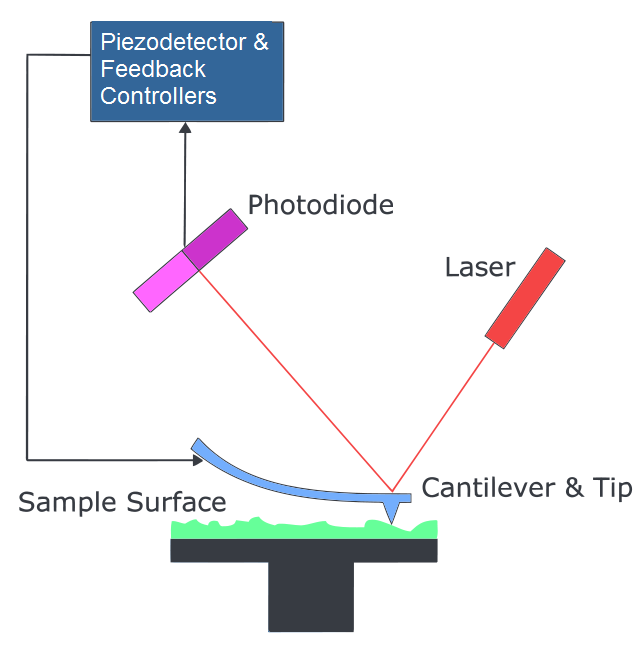
\includegraphics[totalheight=0.5\textwidth, natwidth=640,natheight=640]{640px-Atomic_force_microscope_block_diagram.png}
\caption{Schematic of an atomic force microscope. Note that the size of the text in the figure is comparable to the size of the main text.  Reproduced under Public Domain from Wikimedia Commons\label{AFMblock}}
\end{figure} 



\chapter{Another chapter}\label{ch:results}

\section{Ground State Degeneracy}
In this chapter results of simulations on the dipolar kagome lattice are presented. EFM simulations reveal zero-temperature states lacking domain walls that consist of 3 spins and their negatives. Every ground state obtained through the EFM simulation exhibits a three-sublattice structure with one spin and its negative for each sublattice. The spins alternate in direction along the [1,1,1] direction. 

\begin{figure}
	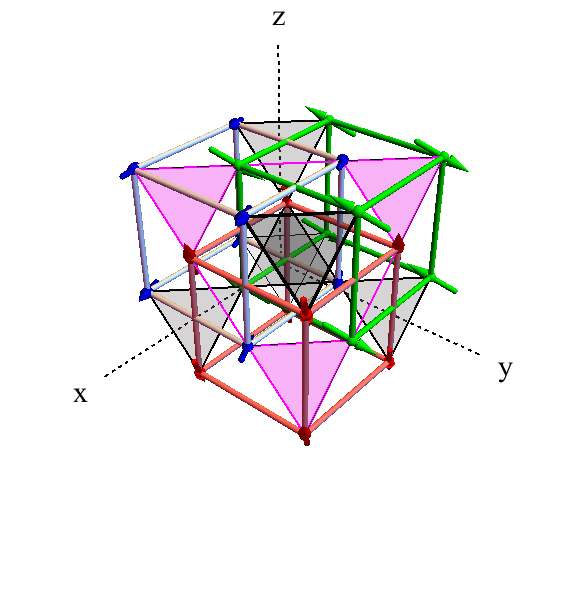
\includegraphics[width=\linewidth]{img/3dfcc.png}
	\caption{A view down the <1,1,1> axis of a 3D FCC lattice with six sub-lattice spin vectors.}
	\label{fig:3dfcc}
\end{figure}

\clearpage
Every ground state configuration obtained through the EFM simulation is characterized by the following set of equations:
\begin{equation}
\label{eqn:rel_a}
\alpha = \sin{\theta} \cos{\phi}
\end{equation}
\begin{equation}
\label{eqn:rel_b}
\beta = \sin{\theta} \sin{\phi}
\end{equation}
\begin{equation}
\label{eqn:rel_c}
\chi = \cos{\theta}
\end{equation}
\begin{equation}
\label{eqn:rel_d}
\delta = (2a^2-1)/2c
\end{equation}
\begin{equation}
\label{eqn:rel_e}
\epsilon = \sqrt(1-a^2-d^2)
\end{equation}

This set of equations acts as elementary building blocks for the components of the spin vectors that exist in the dipolar kagome ground state. The spin vectors may be constructed with this set of equations using the following configuration.

$$\overrightarrow{a} = (\alpha, \beta, \chi)$$
$$\overrightarrow{b} = (\delta, \epsilon, -\alpha)$$
$$\overrightarrow{c} = (-\epsilon, -\chi-\delta, \beta)$$
$$\overrightarrow{d} =-\overrightarrow(a)$$
$$\overrightarrow{e} =-\overrightarrow(b)$$
$$\overrightarrow{f} =-\overrightarrow(c)$$


The set of all possible ground states is therefore characterizable in terms of two parameters: theta and phi. Any theta and phi gives rise to an acceptable ground state of the same energy for a particular lattice size, with the exception of a subset of angles that results in imaginary values for the spin components or undefined division by zero.

\begin{figure}
	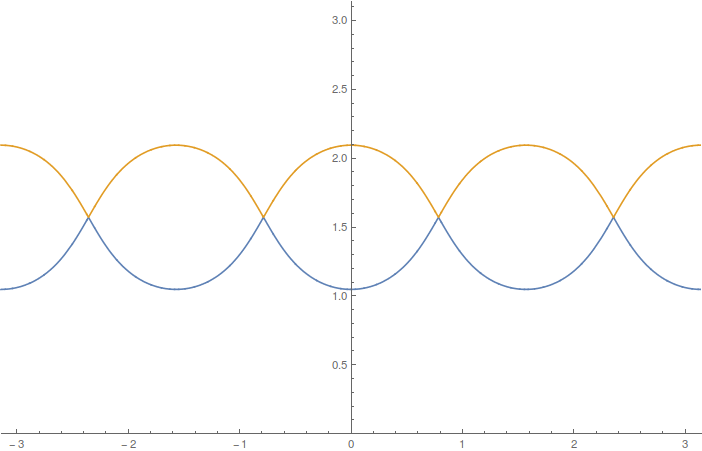
\includegraphics[width=\linewidth]{img/degeneracyplanefull.png}
	\caption{A plane that contains points that allow the construction of valid ground states.}
	\label{fig:degenplanefull}
\end{figure}


Any theta and phi will give rise to a valid ground state of the same energy with the exception of those pairs of theta and phi that lie within the bound region of the graph. Within the bound region of the graph, e = √(1–a²–d²) ∈ ℂ. At each node of each bound area, d = (2a²–1)/2c → ±0/0. Therefore, any choice of theta and phi outside of this region will give rise to a valid ground state of the same energy.

\begin{figure}
	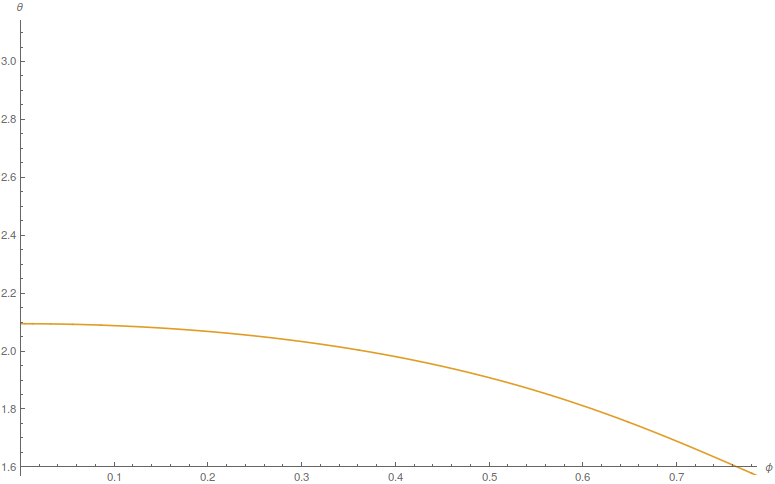
\includegraphics[width=\linewidth]{img/degeneracyplane.png}
	\caption{One section of the original degeneracy plane that is equivalent to all other sections of the plane due to symmetry operations.}
	\label{fig:degenplane}
\end{figure}

It is possible to reduce the size of this graph to 1/16 the size by showing that a state in each portion of the graph is relatable to an analogous state in the other portions of the graph via symmetry operations.
\clearpage

\subsection{Visualization of the Ground State}
\begin{center}
\begin{figure}[ht]
	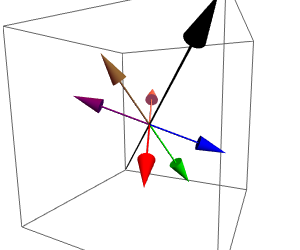
\includegraphics[scale=1.2]{img/samplegs.png}
	\caption{The six sublattice spins conjoined at their ends for clarity and illustration. The vector denoting <1,1,1> axis of symmetry is illustrated in black}
	\label{fig:sampgs}
\end{figure}
\end{center}

By generating the spin vectors described by the !!!equations!!!, a variety of spin configurations can b
\clearpage
\appendix
\chapter{Extra spectra}\label{app:spect}

\section{What should go in an appendix?}

\begin{itemize}
\item raw data, extra images, extra spectra
\item manuals or procedures you've written
\item code
\item detailed explanations of theory that don't fit in your methods chapter
\item etc.
\end{itemize}

%%----------------Bibliography--------------------------------
\addcontentsline{toc}{chapter}{Bibliography}

\bibliographystyle{unsrt_ldw}
\bibliography{bibliography}

\end{document}
